\chapter{Lecture 1}
\lhead{January 12, 2015}
\chead{21-366 Lambda Calculus Lecture 1}

\section{Introduction}
A problem which arises frequently in mathematics is whether a particular statement is true or false. In some cases, this question is easy to answer. The statement $3 + 4 = 7$ can be demonstrated to be true by counting out three stones into a pile, then counting out four more stones. The total number of stones in the pile can be counted as seven. Similarly, we can see that $3 + 4 = 8$ is false.\\

Some statements are less obviously true or false, however. Take the claim that there are a finite number of prime numbers. Consider a list of the first $n$ prime numbers, $p_1,p_2,\ldots,p_n$. Take the product plus one, $P = 1+\prod_{i=1}^{n}p_i$. Now there are two cases: either $P$ is prime, or it is composite. If it is prime, then we have found a prime which is not in our list of the first $n$ primes. If it is composite, then it must be divisible by some prime $q \not=1$. We can see that if $q$ divides $P$, then $q$ divides both $1$ and the product $p_1,p_2,\ldots,p_n$.\\
\margnot{Divisibility Notation}{ If some number $a$ divides some other number $b$ (that is, if $b/a$ is an integer) we write $a|b$.}
\begin{equation*}
  q|(p_1p_2\cdots p_n + 1) \Rightarrow q|(p_1p_2\cdots p_n)\hbox{ and } q|1.
\end{equation*}
If $q$ divides $1$, then $q$ must be $1$, which is a contradiction, so $q$ does not divide the list $p_1,p_2,\ldots,p_n$. This implies that $q$ does not occur anywhere in the list. So we can show that for any list of primes, we can compute another prime which is not in the list. Since we can write an initial list of prime numbers, e.g. $2,3$, this demonstrates that there are an infinite number of prime numbers. Our claim to the contrary is false.\\

If we had not been able to disprove our claim, it is not entirely clear that we could have argued that the claim definitely had to be provable one way or another. (We could have. But bear with me.) Consider a different problem: whether there exists an algorithm which, when given a computer program as input, determines whether the program runs forever, or eventually halts. This problem is known as the \textbf{Halting Problem}\index{Halting Problem}.\\

One attempt at a solution to this problem is to attempt to produce an algorithm which satisfies this specification. Naively, one could attempt to run the program until it either halts, or enters into an infinite loop. We can define an infinite loop in terms of program states. If a program has a repeating pattern of states, then it is in an infinite loop, and will not halt.\\

\margnot{Function Totality}{ A function is called \textbf{total} if it will return some value for every input. Our program $P$ is not total.}

Unfortunately, this fails. Consider a program $P$ which satisfies the following specification. For some other program $S$ and a string $s$, $P(S,s) =$ true if and only if $S$ does not halt on input $s$, and enters an infinite loop otherwise. What happens when we try to run $P(P,P)$? There are two possible cases. If $P$ does not halt on $P$, then $P$ is in an infinite loop. However $P(P,P)$ returns false on the same input program, which is a contradiction. Conversely, if $P$ halts on $P$, then $P$ halts and $P(P,P)$ doesn't, which again is a contradiction. So no such program can exist.\\

In 1936, Alan Turing and Alonzo Church independently solved this problem. Turing invented the notion of a ``Turing Machine,'' which consists of an infinite tape, onto which symbols can be read and written. The machine can decide based on the current symbol and its current state what action to take next. The machine can overwrite the current symbol or move left or right one or more symbols on the tape. What Turing and Church hypothesized was that the class of functions which could be computed by Turing machines was somehow universal. This is the \textbf{Church-Turing Thesis}\index{Church-Turing Thesis}. When people talk casually about a problem being ``computable,'' they usually mean that the problem can be computed on a Turing machine.\\

As an aside, based loosely on the idea of Turing machines is the \textbf{Von Neumann architecture}\index{Von Neumann Architecture} for computers. Almost all modern computers are based on this architecture, or one which expands upon Von Neumann. This means that the question of whether a problem is solvable using Turing machines is equivalent to the question of whether the problem is solvable using modern computers.\\

Aside from Turing's machines, Chuch also came up with a model for computation. His model is the lambda calculus.\\

%John Backus\index{Backus, John} (1977) talks about functional programming\index{Functional Programming}. Hand in lecture notes at the end of the semester, as groups or singularly.
%\margnot{John Backus}{John Backus\index{Backus, John}, 1924-2007 was an American computer scientist who popularized functional programming and led the team which developed the FORTRAN programming language.}

\section{What is Lambda Calculus?}
Lambda calculus is a system which allows us to explore the algebraic properties of computable functions, much in the same way that Turing machines do. It is at its heart fairly simple. There are some things called terms, which we will define below, and some methods for reducing those terms into different terms, which we will discuss at greater length.\\

Turing machines map in an intuitive way to the programming paradigm of \textbf{imperative programming}\index{Imperative Programming}. In both, an instruction pointer is bounced around and the contents of the memory at some designated location is manipulated based on the symbol at the pointer. In each case, program (or machine) state is key. Similarly, lambda calculus also maps to a programming paradigm. This paradigm is \textbf{functional programming.}\index{Functional Programming}\\

The mental model for functional programming (and lambda calculus) is that of reduction. A program consists of a series of definitions. The evaluation of the program is simply the reduction of those definitions until a final state is reached.\\

In the rest of the chapter, we introduce a collection of programs, which are the terms of Lambda calculus. Then we discuss the syntax of these terms.\\

\subsection{Terms of $\lambda$ calculus}
\index{Term|textbf}
{
  Lambda \textbf{terms} are the mechanism by which we produce functions. $\l xX$ represents the substitution of $x$ into $X$, where $X$ is a term in terms of zero or more $x$s. For example, we could write the function $f(x) = x +1$ as $\l x(1 + x)$. Obviously this requires us to define a number of things in terms of lambda calculus that we have not yet defined, like numbers and addition. For now, and until lecture 6, we will assert without evidence that such a thing is possible. This should be satisfactory for now as evidence that lambda calculus can compute things.\\

  \def\tempMargin{\margnot{Alonzo Church}{ Church is best known for the introduction of lambda calculus and the Church-Turing thesis, among other things. He was born in 1903 in Washington D.C., and spent most of his life teaching at Princeton and UCLA.}}
  We have constants, which are names for particular functions, and particular kinds of data. We have variables, like $x$, $y$, and $z$. Church\index{Church, Alonzo}\tempMargin wanted to think about a domain where there is no distinction between data and functions. If $X$ and $Y$ are both terms, then $(XY)$ is a term, read ``$X$ applied to $Y$.'' We could alternately write this as Ap $X Y$. If $X$ is a term and $x$ is a variable, then $(\l x\ X)$ is a term.\\
}

\examplebox{Example: Lambda Terms}{
\begin{eqnarray*}
  x, (\l x\ x), (\l y\ x), (\l x\ (\l y\ x))
\end{eqnarray*}\\
}

\subsection{Currying}
\index{Currying|textbf}
\margnot{Haskell Curry}{ Haskell's name has been immortalized both in the name of the functional programming language Haskell, and in the mathematical operation of currying: converting a function of many variables into a sequence of single variable functions called on each other.}

One intuitive problem that you might have with this model of computation is that there is not an obvious way to describe a function which takes multiple arguments. A model of compuation which cannot represent the addition of two numbers $a$ and $b$ would be a very poor model indeed! At first glance, this problem seems to apply to lambda calculus, with its single fundamental function $\l x(X)$.\\

To resolve this concern, note that if we have a function $\phi(a,b)$, then we can define a second function $\phi(a)$ such that $\phi(a)(b) = \phi(a,b)$. We conventionally write $\phi(a)$ as $\phi_a$. In this way, we can convert a single function of many variables into many functions of a single variable each. So $\phi(a,b)$ becomes $\phi_a(b)$.\\

\subsection{Construction Trees}
We can visually represent the recursive structure of a term by drawing a tree. We call this tree a construction tree\index{Construction Tree}. The construction tree allows us to see the subterms of any term. We define the tree of a constant or a variable is simply tree($x$)$= x$. The tree of a term $(XY)$ would be the tree with the trees of $X$ and $Y$ as subtrees. The tree of a lambda expression $\l xX$ is just the subterm $X$.\\

\begin{center}
  \begin{tikzpicture}[grow'=up]
    \Tree[.$(XY)$ [.{tree$(X)$} ] [.{tree$(Y)$} ] ];
  \end{tikzpicture}
  \hspace{.5in}
  \begin{tikzpicture}[grow'=up]
    \Tree[.$(\l xX)$ [.{tree$(X)$} ] ]
  \end{tikzpicture}
\end{center}
\margnot{Trees Grow Up}{ In Computer Science, trees usually grow down the page from their root node. Our construction trees grow up.}

\examplebox{Example: Construction Tree for $S := (\l x(\l y(\l z((XZ)(YZ)))))$}{
  \begin{center}
    \begin{tikzpicture}[grow'=up]
      \Tree[.$\l x\ \l y\ \l z$ [.$\l y\ \l z$ [.$\l z$ [.$((XZ)(YZ))$ [.$(XZ)$ [.$X$ ] [.$Y$ ] ] [.$(YZ)$ [.$Y$ ] [.$Z$ ] ] ] ] ] ];
    \end{tikzpicture}
  \end{center}
}

%Many terms are defined by recursion on the construction tree.\\

\section{Parenthesis}
\index{Parenthesis|textbf}
At this point in the discussion of the syntax of the lambda calculus, it is worth spending some time talking about parenthesis. We use parenthesis to make explicit and unambiguous what the construction tree for a term looks like. Otherwise, if we came across a term like $\l xXY$, we wouldn't know whether to interpret it as $(\l xX)Y$ or $\l x(XY)$! On the other hand, when we begin to work with longer terms, our notation risks becoming cumbersome if every term must be written with all possible parenthesis. We spend some time now determining the minimum necessary parenthesis necessary to make a term unambiguous so as to save time manipulating cumbersome notation later.

\subsection{Proper Pairings}
A sequence of parenthesis is said to have a \textbf{proper pairing}\index{Proper Pairing} if there exists a bijection $\phi$ from left parenthesis to right parenthesis satisfying two conditions:
\begin{itemize}
  \item $\phi(l)$ is to the right of $l$.
  \item There are no crossings. $(_1(_2)_1)_2$ is bad. $()()$ is okay, and $(_1(_2)_2)_1$ is okay.
\end{itemize}
We claim that the parenthesis of a term are properly paired. We can prove this by induction on the construction tree of a term. If the term is of the form $(x)$, then the parenthesis are properly paired, as there can be no parenthesis inside the variable $x$. If the term is of the form $(XY)$, $(X)$, or $(\l xX)$, then the outermost pair of parenthesis are properly paired if the parenthesis in $X$ and $Y$ are properly paired. We take the case of a single variable as our base case, and see that our induction hypothesis is satisfied, so we are done.\\

\margnot{Connections}{ A sequence of parenthesis can be thought of as a depth-first search of a tree, thinking of a left paren as taking an edge down, and a right paren as taking an edge up.}

We can now also see that if a sequence of parens has a proper pairing, then the sequence is unique. We prove this again by induction. This time, we induct on the number of parenthesis, $n$. If $n = 1$, then it is clear that there is only one proper pairing: $()$.\\

For $n > 1$ we know there must be at least one left paren which begins the sequence. We then have a sequence of zero or more left parenthesis. The first right parenthesis we encounter must be paired with the rightmost left parenthesis:
\begin{equation*}
  (...(_m)_m
\end{equation*}
Observe that there is only one way that this first pairing can be made. $(_m$ must be paired with $)_m$. If this is not the case, then we would have a crossing, which is not allowed in a proper pairing. We remove the $m$ parenthesis, and now we have $2(n-1)$ parenthesis in our pairing. We can then see that the claim is true for all $n$ by induction.\\

\subsection{Checking Whether a Pairing is Proper}
There is a fairly simple algorithm for check whether a pairing is proper. Start with a number $x = 0$ at the left end of the sequence of parenthesis. Every time you encounter a left paren, increment $x$ by 1. Every time you encounter a right paren, decrement $x$ by 1. Throughout this process, if the pairing is proper $n$ will never be negative. The process will terminate with $x = 0$ again.\\

We can prove the correctness of this algorithm as well by induction on the number of pairs of parenthesis, $n$. For $n = 1$, there are only two possible pairings: $()$ and $)($. The first pairing is correct. The sequence of values of $x$ is $0,1,0$. The second pairing has a sequence of $0,-1,0$, so our algorithm claims (correctly) that this pairing is not proper.\\

Now assume that the algorithm is correct for pairings of length $2n$. Our sequence of values for $x$ satisfies the property that the first and last numbers are zero, and that there are no negative numbers in the sequence. We can then add either $0$ or $1$ parens to our list. If we add $1$, then the final value of $x$ will be either $1$ or $-1$, so this make the pairing improper by our algorithm. If we add two parens, and they are unmatched, then TODO: FINISH THIS PROOF